\chapter{Why the Law Needs Bayes}
\label{ch:why}

\begin{quote}\itshape
The theory of probabilities is at bottom nothing but common sense reduced to calculus.
\par\hfill\normalfont Pierre Simon Laplace, 1814
\end{quote}

\section{A court is a decision maker}

A court is asked to do two things. It must find facts, and it must act on them. The first task is a problem of inference: given the evidence, how probable is it that the defendant did what is alleged? The second is a problem of decision: given that probability, and given what is at stake for the parties and for society, what order should the court make? Lawyers have long kept these tasks apart. The jury finds facts and the judge declares law; the standard of proof says how sure the fact finder must be; the remedy follows from liability. Yet the two tasks are linked in every case, because the reason we demand near certainty before a criminal conviction and accept a bare preponderance in a civil claim is that the costs of error differ. That link is the subject of decision theory, and decision theory under uncertainty has one form that avoids sure loss, which is to say one coherent form. It is Bayesian.\index{decision theory}

The Bayesian account of rational action has three ingredients. First, uncertainty about facts is measured by probability, and probabilities are updated in the light of evidence by Bayes' rule. Second, the desirability of consequences is measured by utility, or equivalently by its negative, loss. Third, among the available actions, one chooses the action that maximises expected utility, the average of the utilities of the consequences weighted by their probabilities. Each ingredient can be justified by arguments that do not assume the others: coherence arguments of the Dutch book type for probability \citep{definetti1974}, axioms of preference for utility, and the representation theorems of Ramsey and Savage for the combination \citep{savage1954}. Dennis Lindley spent much of his career showing that these ingredients are not optional extras but the only way to reason that avoids sure loss \citep{lindley1985,lindley2006}.\index{Lindley, Dennis}\index{expected utility}

The aim of this chapter is to set out why that machinery fits the law, to sketch its long history in legal thought, to state the central objections fairly, and to explain the plan of the book.

\section{Three rules and one principle}

Let $G$ denote the proposition that the defendant is guilty, or in a civil case that the claimant's allegation is true, and let $E$ denote the evidence, with $\bar G$ the proposition that $G$ is false. Probability obeys three rules. Convexity says $0 \le \Prob(G \given E) \le 1$, with $\Prob(G\given E) = 1$ when $E$ logically entails $G$. Addition says that for exclusive propositions $A$ and $B$, $\Prob(A \text{ or } B \given E) = \Prob(A\given E)+\Prob(B\given E)$. Multiplication says $\Prob(A \text{ and } B \given E) = \Prob(A \given E)\,\Prob(B\given A, E)$. Lindley liked to say that understanding uncertainty means knowing these three rules \citep{lindley2006}. Bayes' rule is a consequence of the multiplication rule applied twice:
\begin{equation}
\Prob(G \given E) = \frac{\Prob(E\given G)\,\Prob(G)}{\Prob(E\given G)\,\Prob(G) + \Prob(E\given \bar G)\,\Prob(\bar G)} .
\label{eq:bayes}
\end{equation}
It is easier to read in odds form. Writing $\odds(G) = \Prob(G)/\Prob(\bar G)$,
\begin{equation}
\odds(G \given E) = \frac{\Prob(E\given G)}{\Prob(E\given \bar G)} \times \odds(G).
\label{eq:oddsform}
\end{equation}
The ratio in the middle is the likelihood ratio, or Bayes factor, of the evidence. It is the factor by which the evidence should change the odds, and it is the quantity a forensic expert can, at least in principle, speak to without trespassing on the province of the jury. The prior odds $\odds(G)$ summarise everything else.\index{likelihood ratio}\index{Bayes factor}

The decision principle is equally short. Suppose the court must choose between convicting (in a civil case, finding for the claimant), $c$, and acquitting, $a$. Let $L(c, \bar G)$ be the loss from convicting an innocent person and $L(a, G)$ the loss from acquitting a guilty one, with correct decisions carrying zero loss. The expected loss of convicting is $(1-p) L(c,\bar G)$ and that of acquitting is $p L(a, G)$, where $p = \Prob(G\given E)$. Conviction is the better act exactly when
\begin{equation}
p > p^{\ast} = \frac{L(c,\bar G)}{L(c,\bar G)+L(a,G)}.
\label{eq:threshold}
\end{equation}
If convicting the innocent is ten times worse than acquitting the guilty, $p^\ast = 10/11 \approx 0.91$. Blackstone's maxim that it is better that ten guilty persons escape than that one innocent suffer is, read as a statement about the ratio of losses, and \eqref{eq:threshold} turns it into a standard of proof \citep{kaplan1968}. We return to this calculation in Chapter~\ref{ch:standards}, where we show how it organises the criminal and civil standards, the special rules for serious allegations, and Lindley's analysis of sentencing.\index{Blackstone ratio}\index{standard of proof}

\begin{figure}[t]
\centering
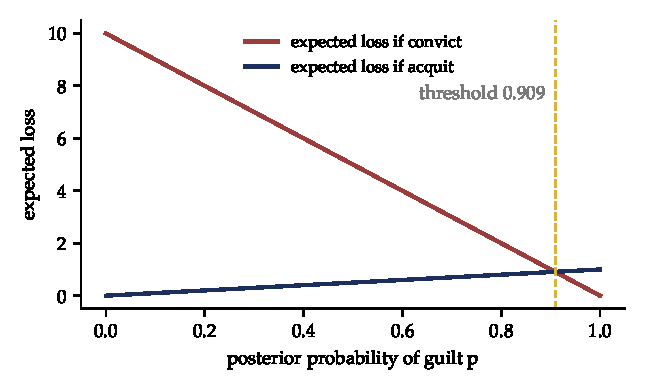
\includegraphics[width=\linewidth]{fig_threshold}
\caption{Expected loss of conviction and acquittal as functions of the posterior probability of guilt, when wrongful conviction is ten times as costly as wrongful acquittal. The two lines cross at the Blackstone threshold $10/11$.}
\label{fig:threshold1}
\end{figure}

\section{A short history of probability in the law}

\subsection{From Bernoulli to Poisson}

Probability and law grew up together. Jacob Bernoulli planned the fourth part of the \emph{Ars Conjectandi} as an application of the new calculus to civil, moral and economic affairs, and his discussion of how arguments combine was framed around legal examples: a man is found murdered, a suspect was seen nearby, he turned pale when questioned, and so on. Leibniz, trained as a lawyer, wrote of degrees of proof and wanted a logic of the probable to assist judges. Nicolas Bernoulli wrote a dissertation on the use of the art of conjecture in law, treating questions such as when a missing person may be presumed dead.\index{Bernoulli, Jacob}\index{Leibniz}

In 1785 Condorcet published his \emph{Essai} on the application of analysis to the probability of majority decisions. The result now called the Condorcet jury theorem says that if each of $n$ jurors independently reaches the correct verdict with probability $q > 1/2$, then the probability that a simple majority is correct tends to one as $n$ grows. If $q < 1/2$ it tends to zero. The theorem is a statement about the binomial distribution: with $n = 2m+1$ jurors, the probability that the majority is right is
\begin{equation}
\Prob(\text{majority correct}) = \sum_{k=m+1}^{n} \binom{n}{k} q^{k}(1-q)^{n-k},
\label{eq:condorcet}
\end{equation}
and the law of large numbers does the rest. Laplace took up the question of how large a majority should be required to convict, and Poisson's \emph{Recherches sur la probabilit\'e des jugements} of 1837 used conviction statistics from the French assize courts to estimate jurors' reliability and the prior probability that an accused was guilty \citep{poisson1837}. The Poisson distribution is named for its appearance in that book, as an approximation to the binomial, although de Moivre had derived the same limit more than a century earlier. It is still fitting that one of the most widely used distributions in science carries the name of an author whose book was about criminal justice.\index{Condorcet jury theorem}\index{Poisson, Sim\'eon Denis}

\begin{casebox}{Poisson and the French juries}
Poisson worked with published statistics on the outcomes of trials in the cours d'assises. Before 1831 a majority of seven to five sufficed to convict, and the law of 1831 required a stronger majority, eight to four. The change in conviction rates gave him leverage to estimate two unknowns: the chance that a juror judges correctly, and the prior probability that a person sent to trial is guilty. His estimates put that prior probability above one half, which is what one would expect if prosecutors screen cases before trial.
\end{casebox}

The nineteenth century then turned against the project. John Stuart Mill called the application of the calculus of probability to testimony and verdicts the real opprobrium of mathematics, and the frequentist revolution in statistics (Venn and Boole in the nineteenth century, Fisher and Neyman in the twentieth), with its insistence that probability is a long run frequency, made it hard to speak of the probability that a particular defendant is guilty. A single crime does not repeat. For much of the twentieth century the official philosophy of statistics had no vocabulary for the question every juror is asked.

\subsection{Wigmore, Turing and Good}

The revival came from two directions. John Henry Wigmore, the great American scholar of evidence, built charts of the logical relations among items of evidence and the propositions they support \citep{wigmore1913}. His charts are graphs in the modern sense, and when Schum, Kadane and others later attached probabilities to them \citep{kadane_schum1996} they became Bayesian networks, the subject of Chapter~\ref{ch:graphs}. At Bletchley Park, Alan Turing and I. J. Good developed the weight of evidence, the logarithm of the Bayes factor, as a practical tool for breaking the Enigma cipher. Good measured it in units Turing had called bans and decibans, and showed how independent items of evidence add on the log scale \citep{good1950,good1979}. After the war Good wrote extensively on the weight of evidence in law and in medicine, and his framework is the natural language for what a forensic scientist reports.\index{Wigmore, John Henry}\index{Turing, Alan}\index{Good, I. J.}\index{weight of evidence}

\subsection{Trial by mathematics}

In 1970 Michael Finkelstein and William Fairley proposed that juries in identification cases be shown how a probability of guilt would change under Bayes' rule for a range of prior probabilities \citep{finkelstein1970}. Laurence Tribe's reply, \emph{Trial by Mathematics}, became one of the most cited articles in American legal scholarship \citep{tribe1971}. Tribe argued that numbers would dwarf soft evidence, that juries could not be asked to state a prior probability of guilt without violating the presumption of innocence, and that a system that acknowledged a quantified risk of convicting the innocent would lose legitimacy. The debate has never quite ended. In England the Court of Appeal in \emph{R v Adams} told trial judges that introducing Bayes' theorem into a jury trial plunges the jury into inappropriate and unnecessary realms of theory and complexity, and in \emph{R v T} it restricted the use of likelihood ratios in footwear evidence where there was no firm statistical base \citep{donnelly2005,fenton2016}. Chapter~\ref{ch:odds} examines these cases closely.\index{Tribe, Laurence}\index{R v Adams}\index{R v T}

The academic response, led by Lindley, Fienberg, Kadane, Dawid, Aitken and Taroni, was to separate two questions that Tribe ran together. Whether a jury should be shown a formula is a question about communication and institutional design. Whether the jury's reasoning ought to obey the rules of probability is a question about rationality. A jury that convicts on evidence that should leave it in doubt is making an error whether or not anyone writes down a number. The value of the Bayesian framework is that it lets us find such errors, explain them, and design procedures that reduce them \citep{fienberg_kadane1983,aitken_taroni2004,dawid2002}.

\section{Lindley's challenge}

Lindley's 1991 paper in the \emph{Journal of the Royal Statistical Society}, \emph{Subjective Probability, Decision Analysis and Their Legal Consequences}, worked through what a court would look like if it took probability and expected utility seriously \citep{lindley1991}. Probability at the start of the trial represents what the fact finder knows before hearing evidence; probability at the end represents what is known after; and the verdict, or the sentence, should be the act that maximises expected utility given the final probability. Lindley showed that a court acting this way might impose some sanction even when the probability of guilt fell below the conventional threshold, because a graduated response can dominate the all or nothing choice between conviction and acquittal. He also offered a new solution to the gatecrasher problem, a puzzle about naked statistical evidence that we take up in Chapter~\ref{ch:standards}.

Lindley went further in conversation and in his later writing. If the task of a court is to combine probabilities with utilities in a coherent way, then that task is a computation, and computations are what machines do well. People would still be needed, he argued, to state the utilities, which express a society's values and cannot be delegated, and to supply the evidence. But the step from evidence and utilities to a verdict could in principle be made by a machine, and made more consistently than by twelve tired jurors or a single overworked judge. His view, as we understand it, was not that machines should replace judges tomorrow, but that the law should be decided by whoever, or whatever, reasons coherently, and that a properly built machine would be held to that standard more easily than a person.\index{Lindley's challenge}\index{artificial intelligence}

We call this Lindley's challenge. It was a provocation in 1991. It is a policy question in 2026, when large language models draft submissions, risk assessment tools inform bail and sentencing in many American states, and some courts experiment with automated triage of their dockets. Chapter~\ref{ch:lindleyai} returns to the challenge after we have built the tools to answer it. Our answer will be that Lindley was right about the structure and that the difficulty lies, as he said, in the utilities and in the evidence. A machine that maximises the wrong expected utility, or that learns its probabilities from biased data, is worse than a careful judge. A machine that is transparent about its probabilities and utilities, and whose computations can be verified, could be better.

\section{Objections and replies}

We state the main objections to Bayesian legal reasoning now, because they recur.

\paragraph{The presumption of innocence forbids a prior} The objection is that asking a fact finder for a prior probability of guilt presupposes that guilt is already somewhat probable, contrary to the presumption of innocence. The reply is that the presumption is a rule about burden and about the evidence that may be used, not a claim that the prior probability is zero. A prior of zero could never be moved by any evidence, so a literal reading would make conviction impossible. A natural Bayesian reading, which we develop in Chapter~\ref{ch:standards}, is that before evidence specific to the defendant is heard, he should be treated as no more likely to be guilty than any other member of the population who could have committed the crime. This gives a prior of the order of $1/N$ where $N$ is the size of that population, and it is the prior used by the defence in \emph{R v Adams}.\index{presumption of innocence}

\paragraph{Probabilities in law are not frequencies} The objection is that a probability of guilt for a single event is meaningless. The reply is that Bayesian probability is a degree of belief, made coherent by the three rules, and that the law already asks fact finders for degrees of belief when it speaks of the balance of probabilities or of proof beyond reasonable doubt. Frequencies enter as evidence about probabilities, through likelihoods and through exchangeability, but they do not exhaust them \citep{definetti1974,lindley2000}.

\paragraph{Numbers overwhelm soft evidence} Tribe's worry was that a precise statistical match probability would crowd out vague but important evidence such as an alibi. The reply is that this is a reason to quantify the soft evidence too, not to ignore the hard evidence. The Bayesian framework is a framework that tells us exactly how an alibi with a modest likelihood ratio should be weighed against a DNA match with an enormous one. In \emph{Adams} the defence did precisely that, and the arithmetic showed that the posterior probability of guilt was far lower than the raw match probability suggested (Figure~\ref{fig:adams1}).

\begin{figure}[t]
\centering
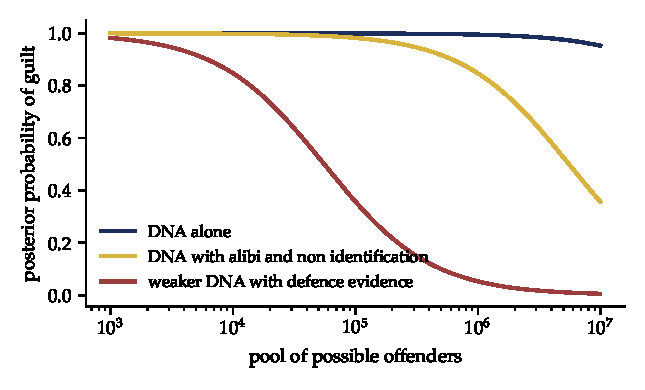
\includegraphics[width=\linewidth]{fig_adams}
\caption{Posterior probability of guilt as a function of the size of the pool of possible offenders, combining a DNA likelihood ratio with defence evidence of the kind presented in \emph{R v Adams}. The defence evidence, with a combined likelihood ratio of about one in thirty six, moves the posterior a long way when the pool is large.}
\label{fig:adams1}
\end{figure}

\paragraph{The law values reasons, not calculations} Courts give reasons, and a verdict that rests on a number may seem to lack them. The reply is that a likelihood ratio is a reason: it says how much more probable the evidence is if the claimant's story is true than if the defendant's is. The Bayesian framework disciplines reasons rather than replacing them. Chapter~\ref{ch:stories} shows how stories, the natural vehicle for legal reasons, can themselves be weighed by their likelihood ratios.

\paragraph{Juries cannot do the arithmetic} This is often true, and it is an argument for better presentation, for the use of verbal scales anchored to likelihood ratios, for graphical aids and for expert guidance, not an argument that the arithmetic is wrong. Fienberg and Kadane gave an early and careful treatment of how Bayesian analyses can be presented in legal proceedings \citep{fienberg_kadane1983}, and the forensic science community has since developed standards for reporting likelihood ratios \citep{aitken_taroni2004}.

\section{The economics of courts}

The Bayesian framework does not stop at the verdict. Courts are institutions with costs. Every hour a judge spends on one case is an hour not spent on another, and every adjournment imposes waiting costs on parties and witnesses. Gary Becker's economic approach to crime treats the probability and severity of punishment as policy instruments chosen to minimise the social cost of crime plus enforcement \citep{becker1968}. The law and economics movement, from Coase and Calabresi to Posner and Shavell, analyses rules of liability by their effects on incentives \citep{coase1960,calabresi1970,shavell1987,posner2014}. Learned Hand's formula in \emph{United States v Carroll Towing}, 159 F.2d 169 (2d Cir.\ 1947), that a party is negligent if the burden of precaution is less than the probability of harm times the gravity of the loss, is an expected cost calculation stated by a judge \citep{posner2014}. We develop these connections in Chapters~\ref{ch:tort} and~\ref{ch:becker}.

Bayesian decision theory supplies the common language. A rule of liability is a decision rule. A standard of proof is a threshold on a posterior probability. A procedural rule, such as a limit on discovery or a rule excluding evidence, is a choice about which information to collect, and its value can be measured by the expected value of sample information. Settlement is bargaining between parties with different posteriors, and the selection of disputes for trial depends on how those posteriors diverge \citep{priest_klein1984}. Even the design of a legal system, common law or civil law, adversarial or inquisitorial, can be read as a choice about how to aggregate information and how to allocate the costs of error.

\section{Machines in the courtroom}

Three technical developments make this book timely.

First, generative and deep learning methods can now approximate posterior distributions for models too complex for classical calculation. In our own work on generative Bayesian computation we train neural networks to map data directly to posterior quantiles, using simulations from the model as training data \citep{polson_sokolov_gbc}. Chapter~\ref{ch:pleadings} applies this approach to Gordon's formal model of civil pleading \citep{gordon1995}, and describes how a network trained on simulated pleadings could estimate the probability that an issue will be decided for the claimant.

Second, large language models can read and summarise legal texts at a scale no human team can match. They can also hallucinate authorities, misstate holdings and express confidence they have not earned. A Bayesian view of these systems asks whether their stated probabilities are calibrated, whether they update correctly on evidence, and whether their errors can be detected.

Third, interactive theorem provers such as Lean have changed what it means to check a proof. Mathematicians now formalise research level arguments so that every step is verified by a small trusted kernel. Lawyers and computer scientists have begun to encode statutes, notably US tax rules on the sale of a principal residence and French family benefits in the Catala language \citep{merigoux2021}, so that the computation of an entitlement can be checked against the text of the law. Chapter~\ref{ch:lean} asks how far this can go. Our view is that verification can certify the logical steps of a legal argument and the arithmetic of a Bayes factor, while leaving the probabilities and utilities, which are matters of judgment, open to argument in the ordinary way.

\section{Comparative perspectives}

The common law and the civil law reason about facts differently. In the English trial the parties control the evidence, the judge is an umpire, and the fact finder must reach a verdict on what the parties choose to present. In the French system the judge directs the inquiry, written evidence dominates, and the criminal court decides according to its \emph{intime conviction}, its inner conviction, a standard that the Code de proc\'edure p\'enale states without numbers. In Chapter~\ref{ch:commoncivil} we model these systems as different strategies for acquiring and aggregating information. The adversarial system is a pair of biased samplers whose biases are supposed to cancel; the inquisitorial system is a single sampler whose bias must be controlled by professional training and appellate review.

These differences have consequences beyond the courtroom. La Porta, Lopez de Silanes, Shleifer and Vishny argued that countries whose legal systems descend from English common law protect investors more strongly than those descended from French civil law, and that this shows up in the size of capital markets and the concentration of ownership \citep{llsv1997,llsv1998}. Their claim has been challenged and refined, but it put legal origin at the centre of development economics. In Africa, colonial history assigned common law to Ghana, Nigeria, Kenya and others, civil law to Senegal, C\^ote d'Ivoire and much of the Sahel, and both to Cameroon. Chapter~\ref{ch:africa} treats this history as a natural experiment and sets out a hierarchical Bayesian model for asking how much of the colonial legacy can be attributed to legal origin. Chapter~\ref{ch:india} turns to India, whose common law courts carry the largest backlog in the world.

\section{Order without the state}

Courts are one way to sustain cooperation. Reputations, kinship and private protection are others. Roger Gould's study of vendettas in nineteenth century Corsica, based on court records, found that revenge was rarer than the folklore suggests and that it was calibrated: it occurred mainly when the original attack involved collaboration or violence against nondisputants, and it was aimed at those who had displayed solidarity with the attacker \citep{gould2000}. Diego Gambetta's study of the Sicilian mafia treats it as an industry selling protection in a market where the state's guarantee of property was weak \citep{gambetta1993}. Both analyses are about signals and inference. A family that avenges a killing signals cohesion; a mafia boss whose threats are credible is one whose type has been revealed. Chapter~\ref{ch:gould} develops these ideas and connects them with Gould's broader argument that conflict is most likely where social rank is ambiguous \citep{gould2003}.

\section{How to read this book}

The book is in seven parts. Part I sets up the tools: decisions, probability and odds, classic cases, Bayes factors, the fallacies, the decision theoretic account of standards of proof, and the kinds of evidence. Part II applies them to English law: tort, mass torts and damages, misrepresentation, contract, family law, the Greensill affair and bankruptcy. Part III treats stories, graphical models and pleadings. Part IV, Statisticians in the Courtroom, covers Fienberg and Kadane and then applied chapters on discrimination, securities, medical evidence, intellectual property and digital evidence. Part V is comparative: common law and civil law, legal origins, Africa, India and arbitration. Part VI is about order without the state. Part VII covers costs and deterrence, antitrust, the costs of the legal system, litigation funding, sentencing and regulation, then verification, the question of artificial intelligence, explainable AI, Hume, a program for reform and the future.

Readers who want the mathematics can find a compact toolkit in Appendix~\ref{app:toolkit}, code for the main calculations in Appendix~\ref{app:code}, and a table of the principal cases in Appendix~\ref{app:cases}. Further appendices give solutions to the exercises, a glossary, a semester teaching plan and a sample examination. Each substantive chapter ends with Notes and Questions, and Appendix~\ref{app:solutions} gives solutions. Some are routine calculations; others are open questions on which we would welcome argument.

\section*{Notes and Questions}
\addcontentsline{toc}{section}{Notes and Questions}
\begin{enumerate}[label=\arabic*.]
\item Using \eqref{eq:threshold}, find the ratio of losses implied by a threshold of $0.95$, and by the civil threshold of $0.5$. What does the second imply about the relative costs of errors for claimants and defendants?
\item Compute the probability that at least seven of twelve jurors are correct, adapting \eqref{eq:condorcet} to $n = 12$, when each is right with probability $0.6$ and votes independently. Repeat for a unanimity rule, taking the probability that all twelve are correct. Why does the Condorcet theorem not apply when jurors deliberate?
\item A suspect is identified by a feature shared by one person in a thousand. The crime was committed in a city of one million adults. With a uniform prior over the city, what is the posterior probability that the suspect is the offender? What additional evidence would raise it above $0.95$?
\item State, in your own words, the difference between the probability of the evidence given innocence and the probability of innocence given the evidence. Construct a short example in which the first is one in a million and the second exceeds one half.
\item Read Tribe's \emph{Trial by Mathematics}. Which of his objections are about rationality and which about institutional design? Which do you find persuasive?
\item Lindley argued that a graduated sanction can dominate the binary choice between conviction and acquittal. Construct a three action example, convict, acquit and an intermediate order, with losses chosen so that the intermediate order is optimal for a range of posterior probabilities.
\end{enumerate}

\section*{Further reading}
Lindley's \emph{Understanding Uncertainty} is the clearest introduction to the Bayesian view \citep{lindley2006}. Aitken and Taroni give the standard treatment of forensic evidence \citep{aitken_taroni2004}. Fienberg's edited report remains the best guide to statistics in American courts \citep{fienberg1989}. Fenton, Neil and colleagues survey Bayes and the law \citep{fenton2016}. On the history, Hacking's \emph{The Emergence of Probability} and Daston's \emph{Classical Probability in the Enlightenment} are indispensable \citep{hacking1975,daston1988}.
